\chapter{Introduction}
Particle accelerators occupy a key role both in fundamental research and in all the applications and industrial processes that uses technology and processes developed initially for the physical research.\\
A number of examples could be named among the spin-offs of accelerators' science, the most notable nowadays is the relevant progress of nanosciences in the last decade, that was made possible by the availability of high-brilliance light sources provided by synchrotrons. In the same way to inquire a much smaller scale are necessaries machines involving higher energies, and the development of the latter will lead the one of the former and so forth.
 Hence in this perspective keep developing the accelerators for the physical research is a fundamental requirement to assure that the cutting-edge technology of today turns into the labware of tomorrow for all the other sciences and the industry, in addition of the contribution that pursuing the fundamental research can give to our understanding of the world of the elementary particles.

%% missing connection

At the moment the most successful model to explain the behaviour of the elementary particles is the \textit{Standard Model}, but it's not conclusive and not able to answer to all the questions still open in particle physics. A milestone in favour of the Standard Model was the observation of the Higgs Boson in 2012, and was made possible by the construction of the \textit{Large Hadron Collider} at CERN\cite{CMS:higgs,ATLAS:higgs,LHC:design}. However the full understanding of the physics at the particle scale still needs to be achieved. Partially this will be realised with the increase of the collision energy of the LHC, but also the International Committee for Future Accelerators (ICFA) consider that the results of LHC needs to be complemented by the results of a lepton collider in the TeV-range\cite{ICFA:linStat}.

The reason of this decision is that according to the standard model the hadrons are particles composed by quarks, that are continously interacting exchanging gluons. This peculiarity cause the collision at high energy not to be between the hadrons themselves, but between partons composing them. In addition, there is no way to know in advance the energy of the partons involved, so it's not possible to know in advance which will be the energy of the collision. For example it is improbable for a parton in the 14 TeV centre-of-mass energy LHC to have much more than 1-2 TeV of energy at the interaction point\cite{LHC:partonDistrib}. On the other hand, the leptons are punctual particles, so the interaction is directly involving the two bullets themselves at a given energy, and the number of possible processes that can take place is definitely smaller. 

This key difference in the behaviour of leptons and hadrons makes hadron colliders \textit{machines for discovery}, because involve all the possible processes that can take place in a wide range of energies, and the lepton machines \textit{machines for precision}, because the reduced number of possible processes guarantees the observation of the events of interest much easier.

\section{Generalities on colliders}

In a collider the rate of observation of  a particular interaction process A is given by
\[
\frac{dN(A)}{dt} = \mathscr{L} \, \sigma(A)
\]
where $\sigma$ is the process cross-section, which depends by the physics of the process itself, and $\mathscr{L}$ is the luminosity, which depends entirely by the machine.
Therefore the figure of merit when it comes to talk about accelerators is the luminosity, which is given by
\[
\mathscr{L} = H_d \frac{N^2}{\sigma_x \sigma_y} n_b f_r
\]
where $N$ is the number of particles per bunch, $\sigma_x$ and $\sigma_y$ are the beam dimensions in the horizontal and vertical plane, $n_b$ is the number of particle per bunch, $f_r$ is the collision frequency of the bunches and $H_d$ is a correction factor that takes in account the non ideality of the collision, such as crossing angle, collision offset, hour glass effect, non gaussian beam profile and so on.

Then becomes obvious try to reach the highest luminosity possible since the events that are going to be studied are rare. This is realised differently according to the design of the accelerating machine in use:
\begin{itemize}
\item linear accelerators (LINACs): present a low repetition frequency, typically lower than hundred of Hz and the beam is passing just once to be accelerated through the machine.
\item circular accelerators (typically synchrotrons): have a higher repetition frequency, up to tenth of KHz, and are keeping the particle beam in orbit for many turns, so can accelerate it over a long period of time
\end{itemize}
After this distinction one could be led to think that the circular machine is the best choice in any case in order to reach high luminosity, but raising the energy of the beam a big issue comes out: the power loss in circular machines due to the emission of synchrotron radiation scales according to the following expression
\[
P \propto \frac{1}{\rho^2} \frac{E^4}{m_0^4}
\]
where $\rho$ is the bending radius of the machine, $E$ is the particle energy and $m_0$ is its rest mass. As can be noted in the table \ref{table_CLIC_ILC_FCC}, the energy loss per turn is a relevant fraction of the beam energy, e.g. for the LEP machine over than 3 GeV were lost per turn, while the record energy per beam was 104.5 GeV. To raise the beam energy and combat the energy loss, the radius of circular machines escalates quickly. Simply scaling LEP, it is possible to show that in order to reach the centre-of-mass energy of 3 TeV, the circumference should be increased to thousands of kilometers \cite{nature:CLIC}.
To solve the issue the development of new lepton colliders is so focusing on two different solutions:
\begin{enumerate}
\item Use muons instead of electrons: this innovative approach reduces the power lost because of the higher mass of the muon compared to the electron, but has to deal with the short life of muons, which is roughly $2 \, \mu s$ in the laboratory frame
\item Limit the losses caused by synchrotron radiation, or increasing the bending radius or abandon the circular topology for the linear one
\end{enumerate}
Also has to be noted that the former technology is rather new and needs to still be fully developed, while the latter profits of the progresses achieved in the last half century mainly in SLAC and KEK on the LINAC technology.

In this perspective a number of project are under study at the moment, of wich the most ambitious are FCC-ee, \textit{Future Circular Collider}, ILC, \textit{International Linear Collider}, and CLIC, \textit{Compact Linear Collider}. The first one consist in a circular collider which is supposed to be placed in a 80-100 km long tunnel before of the installation of the FCC-hh, the other are LINACs even if based on completely different technologies and solutions.  A comparison of the features of these projects in the final stage is presented in the table \ref{table_CLIC_ILC_FCC}, and also LEP is presented as example of circular lepton machine.

\begin{table}
  \centering
    \begin{tabular}{ l c c | c c c }
    \hline
    \hline
    \textbf{Parameter}								& \textbf{LEP2}	&	\textbf{FCC-ee}	&  \multicolumn{2}{c}{\textbf{CLIC}}	&	\textbf{ILC}	\\
    \hline
    $\sqrt{s} \, [GeV]$				& 209	& 350  		&  	500	&  3000	& 500	\\
    $\mathscr{L}_{peak}$  $[10^{34} \, cm^{-2} \, s^{-1}]$	&0.012	& 1.3			&  	2.3	& 	5.9	&1.8		\\
    Total lenght $[km]$						&26.7	& 100		& 13		&  48.4	& 31		\\
    Loaded acc. gradient $[MV/m]$				&		& 			& 80		& 100 	& 31.5	\\
    Bunch population $[10^9]$					& 105	& 170  		&  6.8	& 	3.72	& 500	\\
    Bunch spacing $[ns]$						& 		& 4000	  	&  	0.5	& 	0.5	& 554	\\
    Collision rate $[Hz]$						&  		&  			&  	50	& 	50	& 5		\\
    $\epsilon^*_x \, / \, \epsilon^*_y \, [\mu m]/[nm]$	& 		&  		        &  2.4/25	& 0.66/20	& 10/35	\\  
    $\sigma^*_x\, / \, \sigma^*_y\, [nm]$			& 		&  	3600/70	&  202/2.3	& 40/1	&474/5.9	\\    
    Energy loss per turn $[GeV]$					&  3.34	& 	7.55		& - 		& -		& -		\\
    Power consumption $[MW]$					&  3.34	& 	7.55		& 		& 		& 163	\\
    \hline
    \hline
    %%%%%%%%%%%TABLE STILL TO FIX
    \end{tabular}
  \caption{Comparison of two circular machines, LEP\cite{FCC-ee:leptonCollParam} and FCC-ee\cite{FCC-ee:leptonCollParam,Zimmermann:2057706} and the two projects for linear machines, the fist and last stage of the CLIC implementation \cite{CLIC:cdr} and the final stage of ILC\cite{ILC:tdr} }
\label{table_CLIC_ILC_FCC}
\end{table}



Furthermore a recent interest arose on more compact technologies, e.g. plasma acceleration techniques, but the reliability of such designs still need to be proven in the perspective of creating a fully functional machine that goes beyond the demonstration of the working physical principle.



\section{The CLIC project and the CTF3 facility}

The \textit{Compact Linear Collider} is the project for a linear electron-positron collider capable of reaching a centre-of-mass collision energy of 3 TeV and a luminosity of $2\text{x}10^{34} \, cm^{-2} \, s^{-1}$ in the final stage.

The realisation of such machine implies many technological challenges in order to keep the power consumption and the dimension limited while matching the design goal parameters. These challenges have been faced developing the novel \textit{two-beam acceleration scheme}, in which the idea is to use a high-current and low-energy beam, the \textit{drive beam}, in order to generate the RF power to accelerate a low-current and high-energy beam used for the experiments, named \textit{main beam}. \\
The Drive Beam is produced using a dedicated linac, and then the current is multiplied using a delay loop and two recombination rings, reaching a combination factor of $2\text{x}3\text{x}4=24$. This topology generates the beam with a final frequency of the bunches of 12 GHz, and the reason for this kind of implementation is to reach the highest possible efficiency in the Drive Beam production, in order to shrink the power consumption to the smallest possible. While the biggest challenge for the main beam is reaching the necessary high current, for the Main Beam the hardest challenge is generating a beam with the smallest emittance possible, in order to increase the luminosity of the machine as much as possible.\\
The Main Beam is produced in a separate facility, where a DC-photo gun system provides the initial polarised electron beam, and afterwards part of the beam is used to generate the positron beam. Once both the beams are created, they are sent to the next accelerating stages, which are composed of LINACs to raise the beams' energy and of damping rings to reduce the emittances. 

\vspace{5mm}
(need more details ? maybe a section about the main beam generation ?)
\vspace{5mm}


More information about the Main Beam production and the Drive Beam recombination process can be found in \cite{CLIC:cdr} and about how the working principle have been demonstrated in the CTF3 in \cite{CTF:drive_beam}. 

Once both beams have been produced, both are sent to the Two-beams modules, where the energy of the Main Beam is increased up to the magnitude requested for the experiments. The main beam passes through the PETS, \textit{Power Extraction and Transfer Structures}, and the RF power extracted is transferred to power the accelerating structures for the main beam. The structure of a Two-beams module is exploited in figure \ref{TBM}.



\begin{figure}
\centering

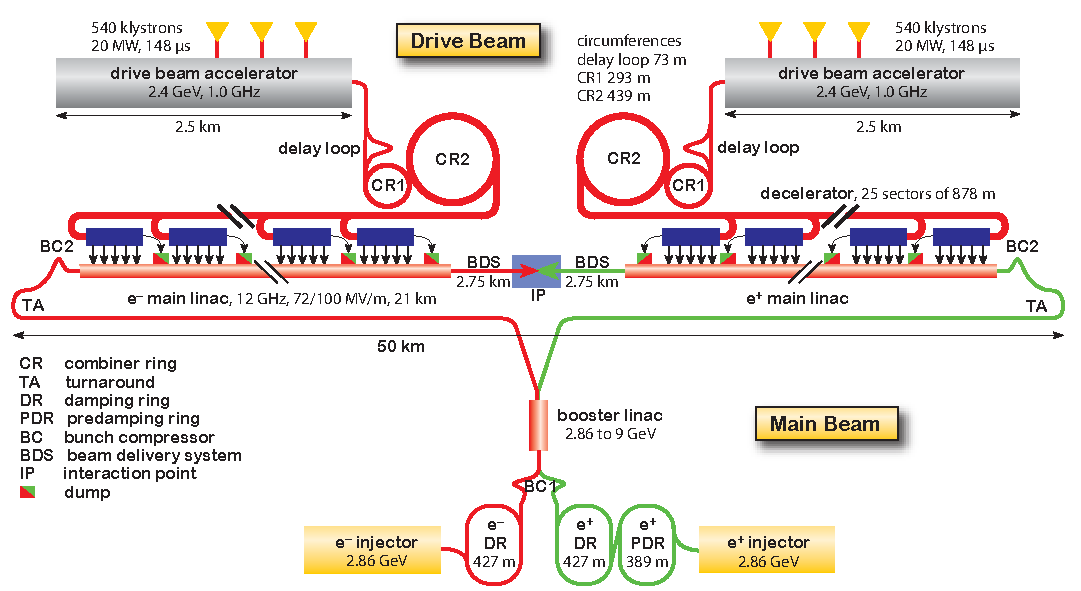
\includegraphics[scale=0.39]{pictures/CLIC_layout_3Tev}
\caption{Layout of the final stage of CLIC}
\label{CLIC_layout}

\hspace{8mm}

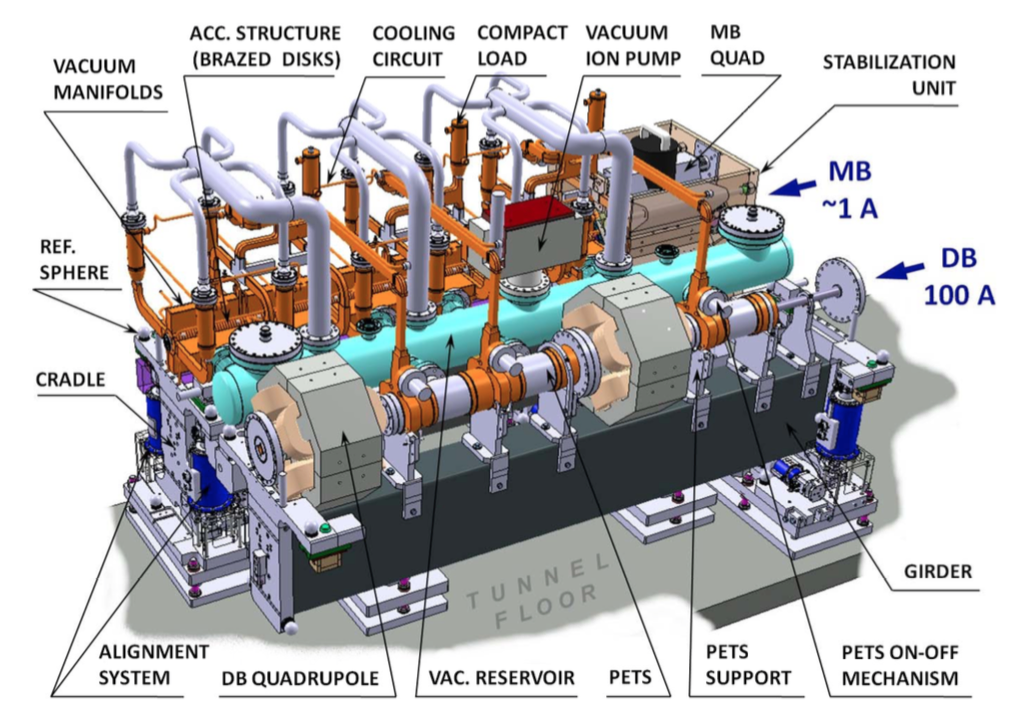
\includegraphics[scale=0.39]{pictures/TBM}
\caption{Design of a Two-beam module. }
\label{TBM}

\end{figure}





\subsection{Physics and staging}

The machine is designed to be built in 3 stages, with a final energy of 3 TeV. The energy of the stages have been chosen in order to offer the possibility to explore both Higgs boson and top quark physics. This modular scheme should allow a physics programme that last for several decades.

Since the CDR\cite{CLIC:cdr} was released just before the discovery of the Higgs boson, the centre of mass energy stages have been reshaped in order to be able to access to interesting measurements, anyway for a given centre-of-mass energy, the energy can be modified by a third with limited loss of performance\cite{CLIC:cdrVol3}, allowing an eventual retuning of the energy of the stages following the results of the last LHC physics campaign.

The energy staging have been chosen as follows, further informations can be found in\cite{CLIC:staging2016,Bozovic-Jelisavcic:2160172}, but the leading idea is to make accessible the Higgs and top physics from the first stage.

The first stage is proposed to be 380 GeV, and it gives access to the Standard model Higgs physics and top-quark physics. The measurements on the former can be conducted through Higgsstrahlung and WW-fusion processes, thereby providing accurate model-indipendent measurements of Higgs couplings to bosons and fermions\cite{Roloff:2210491}; the latter measurements will be focused on the $t\bar{t}$ pair production threshold in the vicinity of $\sqrt{s} = $ 350 GeV.

The second stage is proposed at 1.5 TeV and allows to access new physics phenomena and additional properties of the Higgs boson and the top quark, such as Higgs self-coupling and rare Higgs branching ratios.

The third stage is proposed at 3 TeV and will give direct access to pair-produced particles with mass up to 1.5 TeV or single particles with mass up to 3 TeV. This stage is particularly interesting as test for the BSM theories, since such high energy in a lepton machine makes the observation of new particles much easier than in the LHC.

A further remodulation of these steps is possible after the publication of the results of the run 2 of the LHC, but anyway the advantage of a linear machine in this sense is that the final energy can be reshaped modifying the total length of the machine. In figure \ref{CLIC_map} is shown the track of a possible CLIC build in the Geneva area, in order to give an idea about the order of magnitude of that kind of facility compared to LHC and SPS.

\begin{figure}[h]
\centering

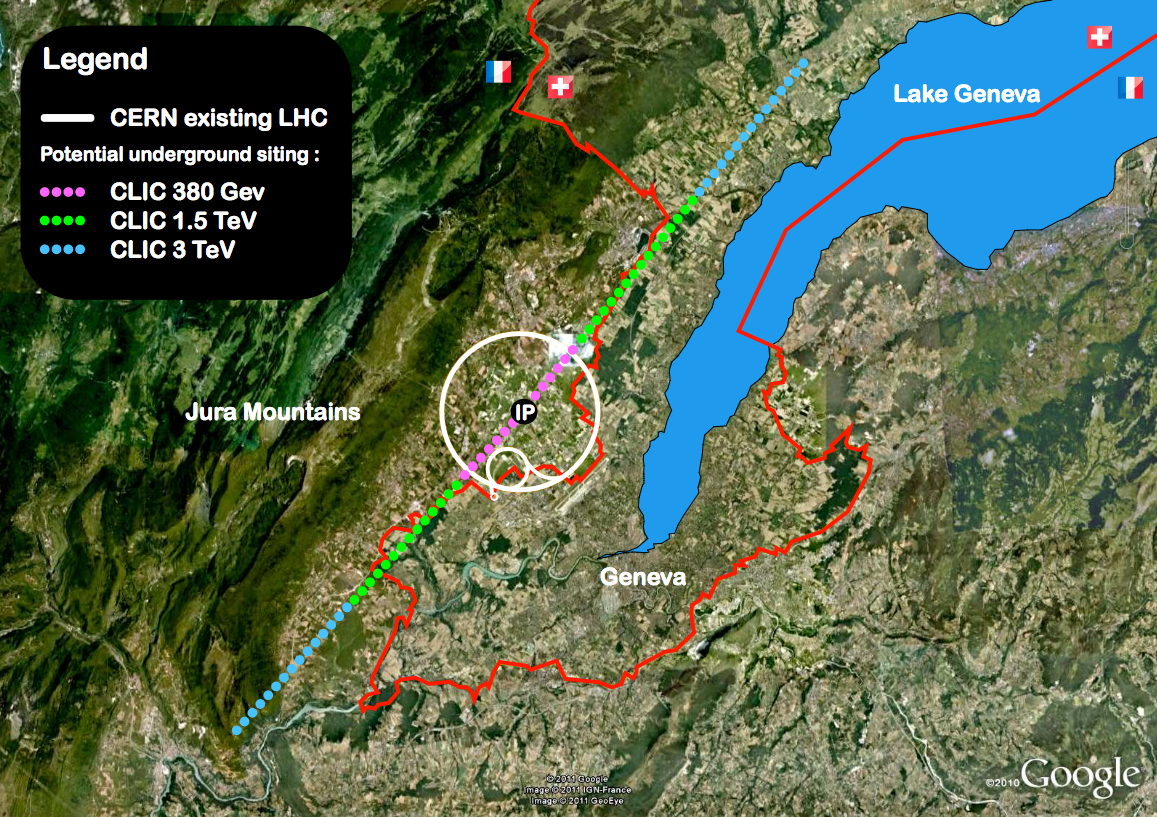
\includegraphics[scale=0.3]{pictures/CLIC_map}
\caption{Map of the CLIC facility, if implemented in the Geneva area}
\label{CLIC_map}

\end{figure}

 

\subsection{Main parameters and main issues}

There are many issues that can affect the performance of a machine like CLIC, and need to be analysed carefully since no similar machine have been built so far. The main issues are:

\begin{enumerate}
\item 100 MV/m accelerating gradient: this requirement comes from the final energy of 3 TeV and the requirement of a maximum length of 50 km
\item Breakdown rate $< 3\text{x}10^{-7}$ breakdowns per pulse per meter: this limitation comes from the limit on design luminosity loss in case of breakdown. Is the aim of this work and will be stressed in detail later
\item Transverse wakefields limitation: wakefields have to be considered because of the short bunch spacing in the bunch train
\item Powering the accelerating structures: no klystrons on the market are able to produce high power pulses 150-200 ns long. This requires the use of pulse compression systems or the two-beam acceleration scheme, that have never built and operated so far. 
\item Generate the drive beam with an efficiency of $97 \%$ in order to contain the power consumption. Also the efficiency of the power transfer between the beams is a key issue in order to reach the energy goal
\item Extremely small beam emittance and size: in order to match the luminosity goal with the typical low repetition rate of a LINAC is necessary to squeeze the beam as much as possible, reaching the goal of 40 and 1 nm at the interaction point in the horizontal and vertical plane. This parameter includes the realisation of a nanometric alignment and vibration containing system 
\end{enumerate}




%%%%% CONSIDER THE REFERENCES [LIST OF CLIC MAIN ISSUES]

Therefore the parameters in the table \ref{table_CLIC_params} have been selected in order to match the design parameters reported in the table \ref{table_CLIC_ILC_FCC} for the top design energy.


\begin{table}[h]
  \centering
    \begin{tabular}{ l c  }
    \hline
    \hline
    \textbf{Description}						& \textbf{CLIC 3 TeV}	\\
    \hline
    Peak luminosity $[cm^{-2} s^{-1}]$				& $2.0\text{x}10^{34}$	\\
    Total site length $[km]$						& 48.4				\\
    Loaded accelerating gradient $[MV/m]$			& 100	\\
    Main LINAC RF frequency	$[GHz]$			& 12	\\
    Charge per bunch $ [nC]$					& $3.7\text{x}10^{9}$ \\
    Bunch separation $[ns]$					& $0.5$ \\
    Bunches per train							& $312$ \\
    Beam pulse duration $[ns]$					& $156$ \\
    $\epsilon^*_x \, / \, \epsilon^*_y \, [\mu m]/[nm]$	& $0.66/20$ \\  
    $\sigma^*_x\, / \, \sigma^*_y\, [nm]$			& $40/1$	\\
    
    \hline
    \hline
    %%%%%%%%%%%TABLE STILL TO FIX
    \end{tabular}
  \caption{CLIC main parameters in the final stage}
\label{table_CLIC_params}
\end{table}


%%%%% TELL ABOUT THE KLYSTRON OPTION, non credibile, ma forse per energie basse ....

%%%%% COMMENTO SUI PARAMETRI





\subsection[CTF3]{The CLIC Test Facility 3}

In lobortis augue porta dui venenatis sollicitudin. In sagittis quis ipsum non dictum. Sed tempus, quam non vehicula dictum, mauris nisl posuere metus, eu lobortis odio risus at dui. Nullam non ante vulputate nulla ultrices euismod eu a diam. Cum sociis natoque penatibus et magnis dis parturient montes, nascetur ridiculus mus. Nulla nec augue a risus viverra mattis. Ut tincidunt egestas nulla at semper. Fusce pretium, leo quis consectetur viverra, arcu lectus ornare leo, quis commodo ex risus sit amet velit. Nullam finibus lorem in mi tincidunt, sed feugiat lectus tincidunt. In hac habitasse platea dictumst. Sed quis auctor odio, at sodales nunc. Donec vulputate massa sit amet dolor sollicitudin, vel pretium quam scelerisque. Nullam et massa eleifend, venenatis ante vitae, ornare libero. Suspendisse potenti. Nam ante lacus, porttitor vel turpis quis, pellentesque auctor velit.

In lobortis augue porta dui venenatis sollicitudin. In sagittis quis ipsum non dictum. Sed tempus, quam non vehicula dictum, mauris nisl posuere metus, eu lobortis odio risus at dui. Nullam non ante vulputate nulla ultrices euismod eu a diam. Cum sociis natoque penatibus et magnis dis parturient montes, nascetur ridiculus mus. Nulla nec augue a risus viverra mattis. Ut tincidunt egestas nulla at semper. Fusce pretium, leo quis consectetur viverra, arcu lectus ornare leo, quis commodo ex risus sit amet velit. Nullam finibus lorem in mi tincidunt, sed feugiat lectus tincidunt. In hac habitasse platea dictumst. Sed quis auctor odio, at sodales nunc. Donec vulputate massa sit amet dolor sollicitudin, vel pretium quam scelerisque. Nullam et massa eleifend, venenatis ante vitae, ornare libero. Suspendisse potenti. Nam ante lacus, porttitor vel turpis quis, pellentesque auctor velit.